\chapter*{Wprowadzenie}
\addcontentsline{toc}{chapter}{Wprowadzenie}
%  \begin{figure}
%   \centering
% \includegraphics[width=340px]{./diagramy/poco.pdf}
%   \caption{Zarysowanie problemu}
%  \end{figure}
\begin{figure}[h]
 \centering
 \includegraphics[width=400px]{../diagramy/poco.pdf}
 % poco.pdf: 596x842 pixel, 72dpi, 21.03x29.70 cm, bb=0 0 596 842
 \caption{Przedstawienie problemu}
 \label{fig:poco}
\end{figure}

% jaka będzie wartość dodana tego co zrobimy
% cała ścieżka Informatyka -> nasza praca
% celem naszym było usystematyzować pracę nad systemami dla sumerologów

% nasza ścieżka: Informatyka -> Inżynieria oprogramowania -> różne podejścia -> domain-specific podejście -> domain specific language

Główną gałęzią informatyki jest tworzenie oprogramowania, służącego człowiekowi w rozwiązywaniu różnych problemów i wspomaganie go w jego działalności. Praktyczną stroną tego procesu zajmuje się inżynieria oprogramowania, która wyróżnia wiele podejść do samego sposobu programowania. Są to między innymi programowanie zorientowane obiektowo, ktore zakłada, że wszystko jest obiektem; programowanie zorientowane aspektowo, które zakłada, że wszystko jest aspektem oraz programowanie zorientowane na językowo, które polega na stworzeniu języka odpowiadającego domenie problemu (domain specific language) a następnie rozwiązuje go w tym języku. Polega to na tym, że projektuje się i implementuje język, w którym opisywanie problemów dziedziny jest znacznie prostsze i bardziej naturalne. Dzięki temu mogą je opisywać nie tylko programiści ale także ludzie związani tylko z konkretną dziedziną. 
Zazwyczaj do konkretnego problemu jedno z podejść pasuje zdecydowanie bardziej niż inne. W niniejszej pracy zdecydowałyśmy się zastosować programowanie zorientowane na język w celu usystematyzowania pracy nad systemami dla sumerologów. 


 
Niniejsza praca dotyczy problemu przetwarzania baz danych tabliczek sumeryjskich przez osoby nieznające specyficznych dla baz danych języków zapytań.


Istnieje wiele baz danych zawierających teksty odczytane z tabliczek sumeryjskich (najbardziej znana - CDLI zawiera ich prawie 225 tys.). Sumerolodzy zajmują się badaniem i przetwarzaniem tych tekstów, jednak wyszukiwanie interesujących ich tabliczek jest dosyć niewygodne. Wynika to przede wszystkim z nieznajomości specyficznych dla baz danych języków zapytań. 
Większość serwisów internetowych udostępnia formularze ułatwiające wprowadzanie kryteriów wyszukiwania, jednakże mają one ograniczone możliwości (nie pozwalają na skomplikowane konstrukcje). Dlatego istnieje potrzeba stworzenia narzędzia, które będzie łączyło w sobie jak największą siłę wyrazu i łatwość użycia przez osoby znające jedynie dziedzinę problemu. Celem projektu przedstawionego w niniejszej pracy jest zaprojektowanie i implementacja języka Tablets Query Language (TQL) spełniającego powyższe wymagania. 

TQL jest podstawą do tworzenia podobnych języków wyszukiwań dostosowanych do potrzeb innych grup ludzi, np. językoznawców.
Większość programów ułatwiających tworzenie zapytań jest skomplikowana, daje ograniczone możliwości lub jest przystosowana głównie do przetwarzania danych liczbowych. Tablets Query Language rozwiązuje te problemy: jest prosty i intuicyjny, przystosowany głównie do tekstów, minimalnie zmniejsza siłę wyrazu oraz łatwo go rozbudowywać. 

%Język TQL jest nakładką na inne języki (m.in. SQL). 
Zgodnie z paradygmatem języków dziedzinowych (Domain Specific Languages, DSL) TQL jest tłumaczony do innych, istniejących wcześniej języków zapytań bardziej ogólnego zastosowania (np. SQL).
% TQL jest jednym z języków dziedzinowych (Domain Specific Languages, DSL). 
W związku z tym dla każdego sposobu reprezentacji danych należy skonstruować translator, 
którego zadaniem będzie przetłumaczenie zapytania. 
% Dla każdego z nich, w zależności od reprezentacji danych, należy skonstruować translator, 
% którego zadaniem będzie przetłumaczenie zapytania. 
W ramach niniejszej pracy przedstawione zostaną dwa przykładowe translatory.
